\documentclass[12pt,a4paper]{report}

%----------------------------------------------------------------------------------------
%   PACKAGES
%----------------------------------------------------------------------------------------
\usepackage[francais]{babel} % French language package
\usepackage[utf8]{inputenc} % UTF8
\usepackage[T1]{fontenc} % acute french accents
\usepackage[pdftex]{graphicx} % figures
\usepackage[hidelinks]{hyperref} % hyperlinks
\usepackage[dvipsnames]{xcolor} % colors
\usepackage{amsthm} % mathematical symbols
\usepackage{pdfpages}

\usepackage{titlesec}
\titleformat{\chapter}[display]
{\normalfont\huge\bfseries}{\chaptertitlename\ \thechapter}{20pt}{\Huge}
\titlespacing*{\chapter}{0pt}{-50pt}{40pt}

\makeatletter
\setlength{\@fptop}{0pt}
\makeatother
\begin{document}
%----------------------------------------------------------------------------------------
%   TITLE PAGE
%----------------------------------------------------------------------------------------
\begin{titlepage}
\newcommand{\HRule}{\rule{\linewidth}{0.5mm}} % Defines a new command for the horizontal lines
\center

%----------------------------------------------------------------------------------------
%   LOGOS SECTION
%----------------------------------------------------------------------------------------

\includegraphics[scale=0.5]{images/umLogo.png} % Université de Montpellier Logo
\hspace{\fill}

\includegraphics[scale=0.25]{images/fdsLogo.jpg} % Faculté de Sciences Logo

%----------------------------------------------------------------------------------------
%   HEADING SECTIONS
%----------------------------------------------------------------------------------------
\textsc{\LARGE M1 Informatique AIGLE}\\[1cm]
\textsc{\Large \textbf{HMIN204}}\\[0.25cm]
\textsc{\large Conduite de Projet}\\[0.5cm]

%----------------------------------------------------------------------------------------
%   TITLE SECTION
%----------------------------------------------------------------------------------------
\HRule \\[0.4cm]
{ \huge \bfseries Méta-Rapport du TER}\\[0.4cm]
\HRule \\[0.5cm]

%----------------------------------------------------------------------------------------
%   AUTHORS AND SUPERVISORS SECTION
%----------------------------------------------------------------------------------------
{ \huge \bfseries Groupe \textsc{Bajonim}}\\[0.4cm]
\begin{minipage}{0.4\textwidth}
\centering \small
\textbf{Bachar \textsc{Rima}}, \\ \href{mailto:bachar.rima@etu.umontpellier.fr}{bachar.rima@etu.umontpellier.fr}\\ % Student
\textbf{Joseph \textsc{Saba}}, \\ \href{mailto:joseph.saba@etu.umontpellier.fr}{joseph.saba@etu.umontpellier.fr}\\ % Student
\textbf{Tasnim \textsc{Shaqura}}, \\ \href{mailto:tasnim.shaqura@etu.umontpellier.fr}{tasnim.shaqura@etu.umontpellier.fr}\\ % Student
\end{minipage} \\[0.8cm]

\begin{center}

\emph{Responsable de l'UE:} \\
Eric \textsc{Bourreau} % UE Supervisor
\end{center}

%----------------------------------------------------------------------------------------
%   DATE SECTION
%----------------------------------------------------------------------------------------
{\large 22 mai 2019}\\[1cm]
\hspace{\fill}
\vfill % Fill the rest of the page with whitespace
\end{titlepage}

\tableofcontents

\chapter{Sujet}
Les logiciels sont actuellement omniprésents dans tous les aspects de notre vie quotidienne; archiver leurs codes source paraît ainsi une tâche primordiale. En effet, le code source d'un logiciel constitue un artefact logiciel fondamental dans le domaine des connaisances scientifiques, culturelles, et techniques. D'autre part, le code source est facilement lisible et compréhensible par les humains, et peut être transformé en fichiers exécutables. À ce titre là, des plateformes ont déjà été proposées, telles que \texttt{The Internet Archive} et \texttt{UNESCO Persist}. Toutefois, ces plateformes se concentraient plutôt sur la préservation des fichiers exécutables.

\texttt{Software Heritage} est un projet visant la préservation du code source des logiciels \textit{open-source}, publiquement accessibles par quiconque. L'architecture de \texttt{Software Heritage} consiste en un \textit{framework} permettant de retrouver les codes source publiquement accessibles depuis n'importe quel plateforme d'hébergement et de les ingérer dans l'archive de \texttt{Software Heritage}. En particulier, les \textbf{Listers} en constituent une partie centrale; il s'agit de crawlers configurés pour parcourir des dépôts de code source et reporter leur ingestion à d'autres composants de l'architecture. En outre, les plateformes d'hébergement embarquent le code source dans des dépôts à structures différentes, ce qui nécessite la création d'un \textbf{Lister} dédié pour chaque platforme. Actuellement, tous les \textbf{Listers} développés ont été créés uniquement par l'équipe de \texttt{Software Heritage}. Les \textbf{Listers} ont été développés pour les plateformes d'hébergement les plus populaires (\texttt{Github}, \texttt{Bitbucket}, $\dots$).

Dans le cadre de ce projet, encadré par Jessie Carbonnel, nous avons cibler la plateforme d'hébergement \texttt{Launchpad} afin de lui développer son \textbf{Lister} correspondant. Ainsi, les objectifs de ce TER peuvent être énumérés de la manière suivante :
\begin{itemize}
  \item Lire/comprendre les articles et tutoriels écrits par l'équipe de \texttt{Software Heritage} ;
  \item Analyser différentes plateformes d'hébergement afin d'en cibler une ;
  \item Concevoir et développer un \textbf{Lister} pour la plateforme choisie ;
  \item Répliquer localement l'environnement de \texttt{Software Heritage} afin de tester le \textbf{Lister} développé ;
  \item Faire une \textit{Pull Request} afin d'intégrer le \textbf{Lister} testé au dépôt de développement de \texttt{Software Heritage} sur \texttt{GitHub}.
\end{itemize}

\chapter{Planning}
Dans ce chapitre, nous présentons les versions prévisionnelle et finale du \textbf{diagramme de} \texttt{Gannt}, ensuite nous en élaborerons un comparatif.

\section{Planning Prévisionel}
\begin{figure}[!ht]
\hspace*{-3.5cm}
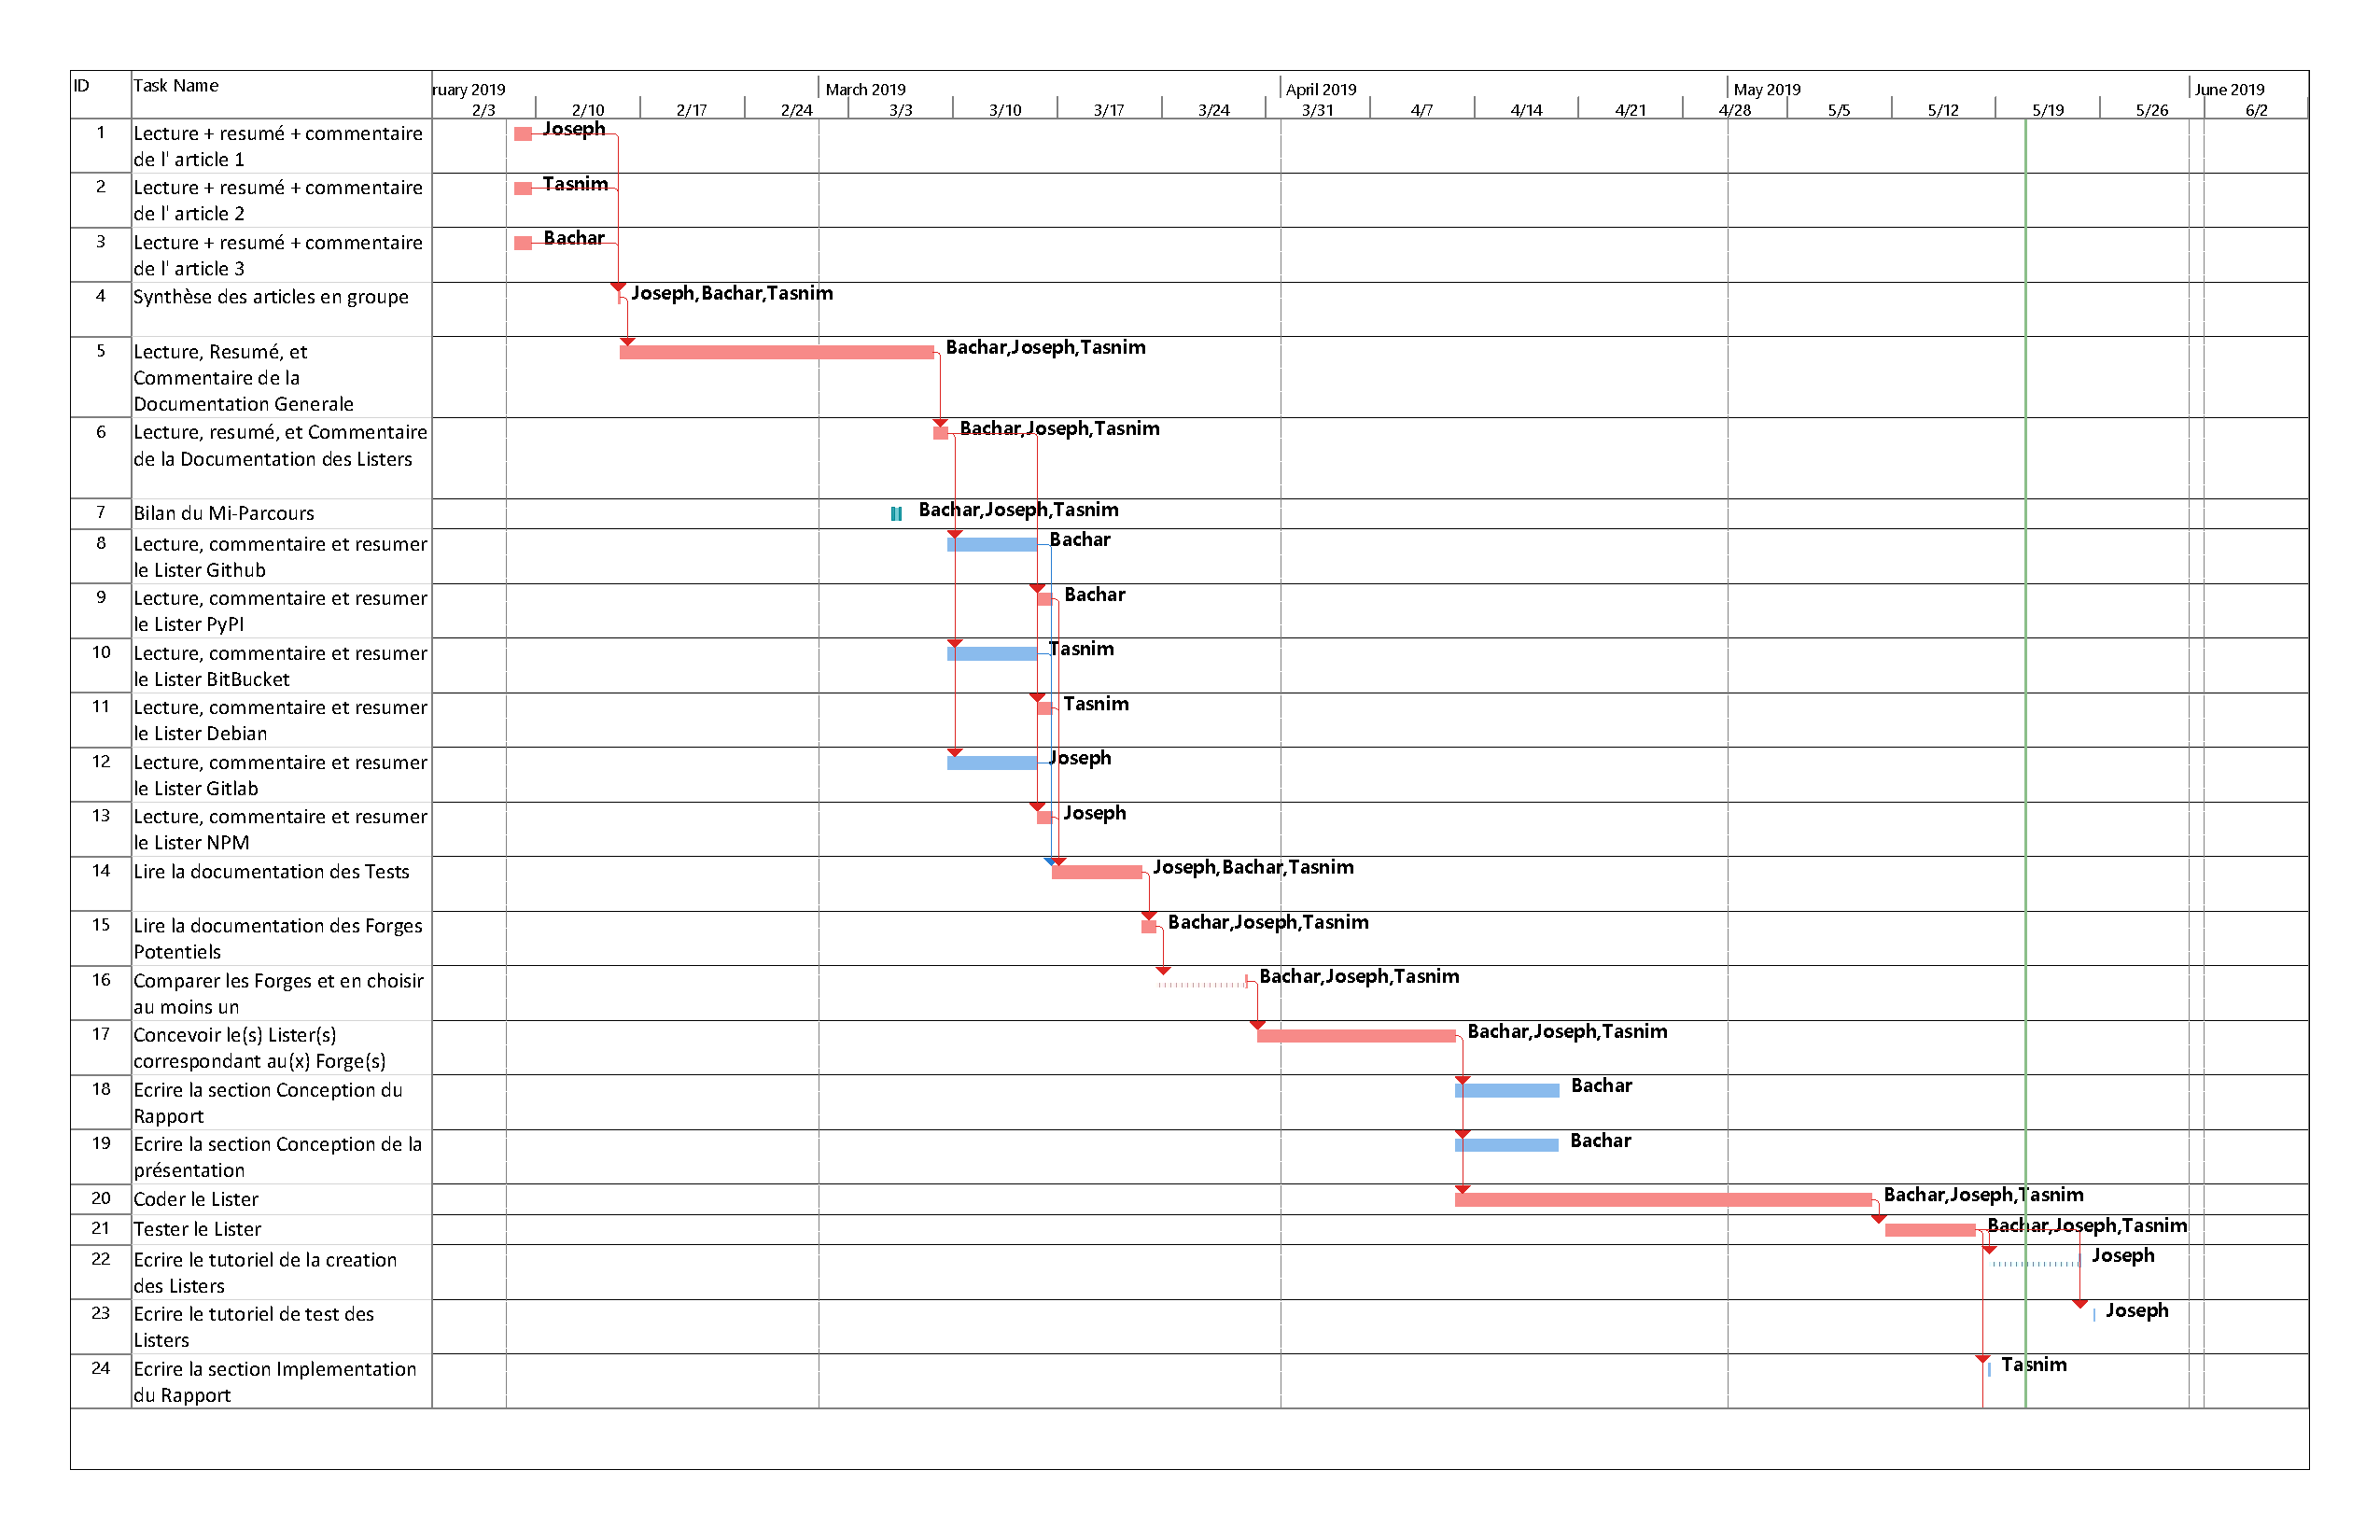
\includegraphics[scale=0.48]{pdfs/feuille_de_route.pdf}
\end{figure}

\begin{figure}[!ht]
\hspace*{-3cm}
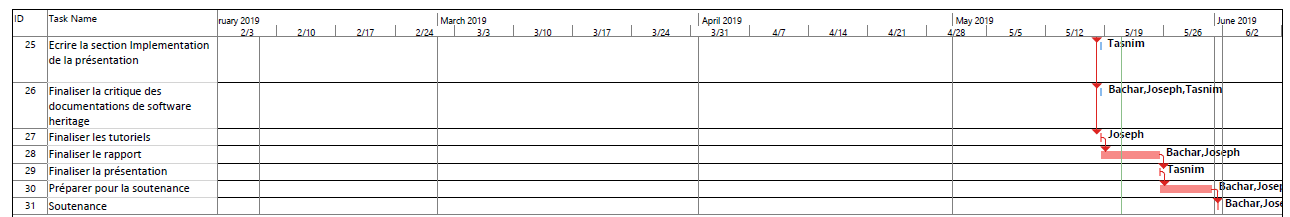
\includegraphics[scale=0.57]{images/planning_prev_p2.PNG}
\caption{Planning prévisionel}
\end{figure}

\subsection{Notes sur le planning prévisionnel}
Lors de la mise en place du \textbf{diagramme de} \texttt{Gannt}, la définition des tâches était trop généraliste et leur regroupement explicite était absent.

\newpage

\section{Planning Final}
\begin{figure}[!ht]
\hspace*{-3.5cm}
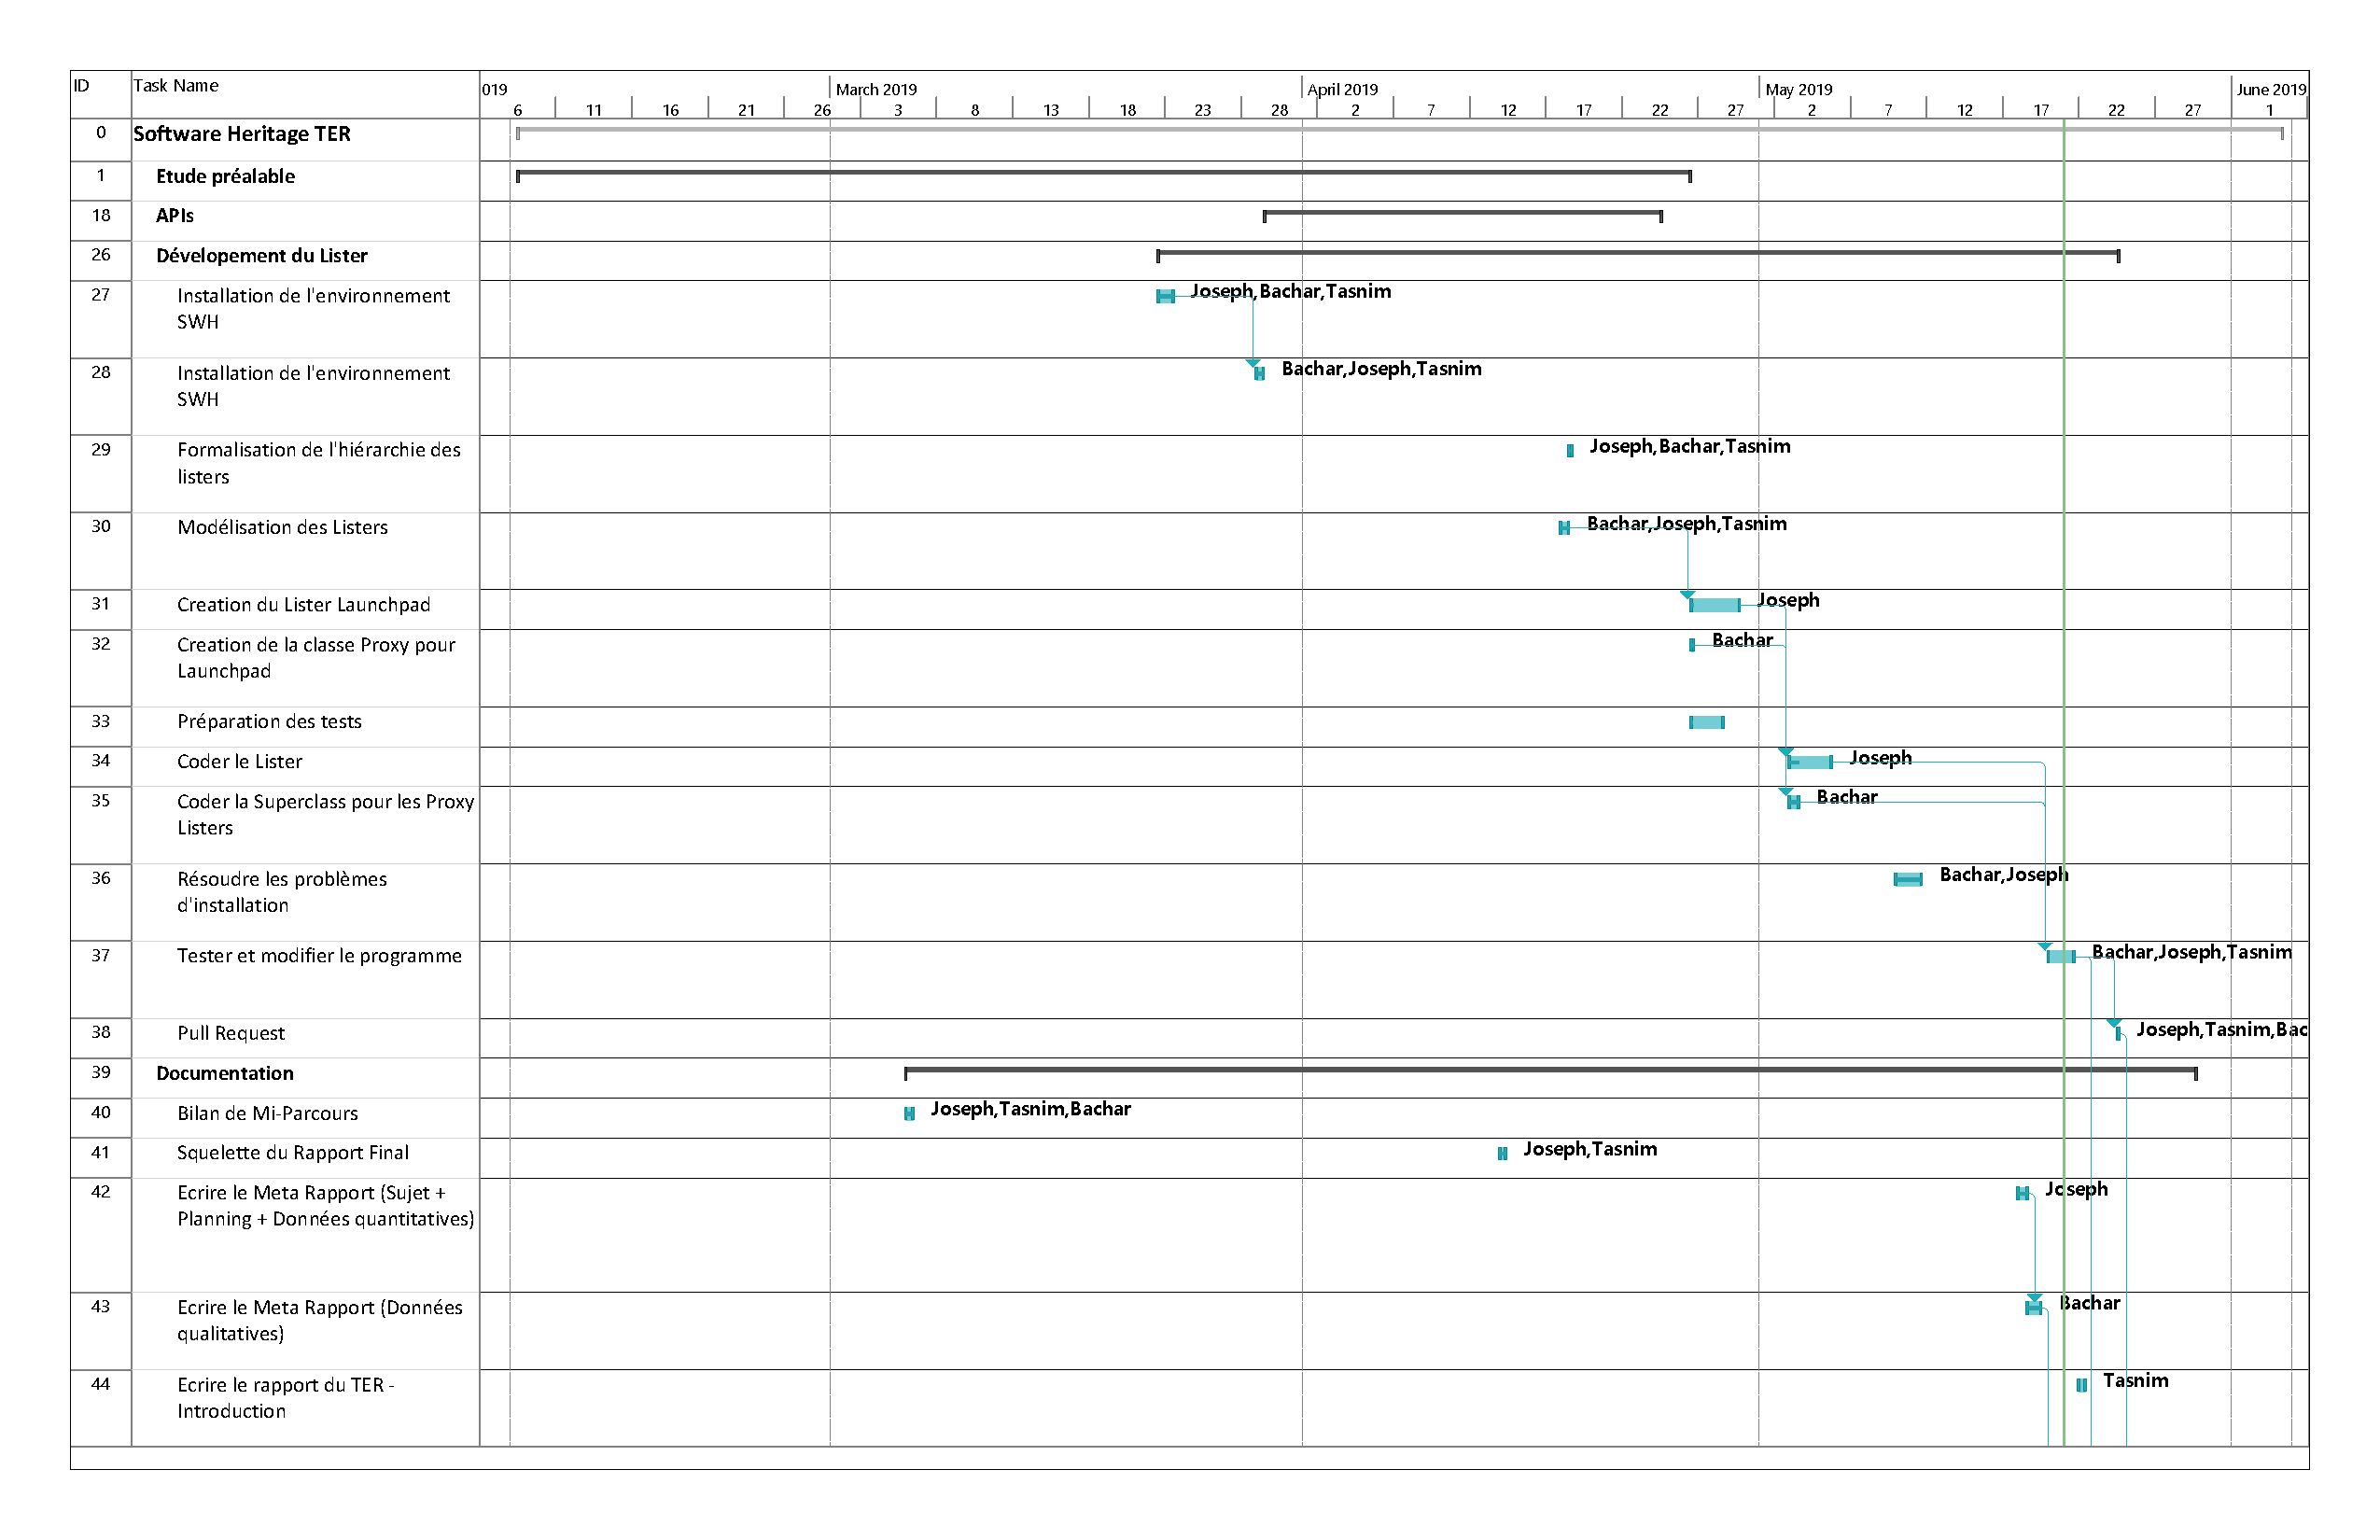
\includegraphics[scale=0.48]{pdfs/planning_final_summary.pdf}
\end{figure}

\begin{figure}[!ht]
\hspace*{-3.5cm}
\includegraphics[scale=0.48,page=2]{pdfs/planning_final_summary.pdf}
\caption{Planning final}
\end{figure}

\newpage

\subsection{Notes sur le planning final}
Au fur et à mesure de notre avancement, pour mieux refléter la structure du projet et pour être cohérent avec la théorie acquise au sein du module de conduite de projet, nous avons regroupé nos tâches de la manière suivante :
\begin{description}
  \item [Étude préalable :] la plus grande section du projet. Elle regroupe toutes les tâches de lecture et de recherche qui ont permis de nous familiariser avec l'architecture et l'environnement de \texttt{Software Heritage} en général, et l'implémentation des différents \textbf{Listers} prédéfinis en particulier.
  \item [APIs :] la section regroupant les tâches de recherche d'une plateforme d'hébergement de code ayant une \textbf{API} adaptée à nos besoins et qui sera exploitée par les tâches de développement.
  \item [Lister :] la section regroupant les tâches de conception, développement et test du \textbf{Lister}.
  \item [Documentation :] la section regroupant les tâches de rédaction des rapports et de la présentation pour la soutenance.
  \item [Soutenance :] la section regroupant les tâches d'entraînement pour la soutenance.
\end{description}

\section{Comparaison des plannings}
La date de délai du planning prévisionnel occurrant assez tôt par rapport au lancement du module TER, nous n'avions pas eu le temps de récolter les informations nécessaires pour raffiner la répartition des tâches. Par conséquent, n'ayant pas une estimation concrète des différentes phases du développement du livrable, nous nous sommes contentés d'adopter une approche initiale généraliste en vue de la spécialiser au fur et à mesure de notre avancement.

Après, la récolte continuelle d'informations nous a permis de raffiner notre planning prévisionnel. Effectivement, certaines tâches ont été spécialisées et d'autres ont été ajoutées, par exemple :
\begin{description}
  \item [tâche spécialisée :] \og \textit{Coder le lister} \fg~ spécialisée en \og \textit{Création du ProxyLister \texttt{Launchpad}} \fg , \og \textit{Création de la classe Proxy pour \texttt{Launchpad}} \fg, \og \textit{Création de la superclasse des ProxyListers} \fg, et \og \textit{Création de la superclasse des Proxy} \fg ;
  \item [tâche ajoutée :] \og \textit{résoudre les problèmes d'installation de l'environnement de \texttt{Software Heritage}} \fg.
\end{description}

Ces adaptations sont majoritairement dues aux raisons suivantes :
\begin{itemize}
  \item la durée de la recherche d'une plateforme d'hébergement de code ayant une \textbf{API} adaptée à nos besoins, imprévisible sans comprendre le fonctionnement de \texttt{Software Heritage} permettant de formuler les requis nécessaires ~;
  \item la maintenance et la mise à jour de la plateforme \texttt{Software Heritage}, nous empêchant d'estimer correctement la durée des tests ;
  \item le croisement des dates de délai d'autres UE\footnote{méritant eux aussi un temps conséquent pour les compléter}, avec celles définies pour le TER, nous empêchant de suivre minutieusement le planning prévisionnel défini.
\end{itemize}

\section{\textit{Features et issues}}
Actuellement, le \textbf{Lister} a été conçu, implémenté et intégré à l'architecture d'une instance locale de \texttt{Software Heritage}. Malheureusement, la plateforme étant actuellement en maintenance et non disponible pour un usage local, nous n'avons pas encore pu exécuter les tests unitaires définis. Toutefois, après avoir communiqué avec l'équipe de développement de \texttt{Software Heritage} via un canal IRC dédié, nous nous sommes renseignés sur la date de reprise d'activité de la plateforme. Par conséquent, nous essayerons, d'ici la date de délai de notre travail de TER, de finaliser les tests, une fois la plateforme ait repris son activité.

Enfin, nous ferons un \textit{Pull Request} auprès du dépôt \texttt{GitHub} du développement de \texttt{Software Heritage}, afin d'intégrer notre \textbf{Lister} à leur projet; nous serons ainsi la première équipe communautaire (\textit{i.e. hors l'équipe de développement de \texttt{Software Heritage}}) à avoir effectué une contribution.\\
\noindent Nous estimons environ 9 à 10 heures de travail pour finaliser ces deux étapes.

\chapter{Organisation}
\section{Stratégie de développement et répartition des tâches}
\subsection{Analyse du risque}
Afin d'élaborer une stratégie de développement performante et pertinente, nous avons commencé notre démarche par l'analyse des risques associés au projet. Par conséquent, nous nous sommes retrouvés avec un profile de risque normal. En effet, notre équipe étant composée de trois personnes a largement minimisé les problèmes de transfert de connaissance. D'autre part, les difficultés liées à l'apprentissage des technologies avaient des conséquences non négligeables sur le temps d'adaptation de l'équipe au fonctionnement de \texttt{Software Heritage}.
Par ailleurs, le projet n'étant pas créé \og \textit{from scratch} \fg~ a diminué suffisamment sa taille et son temps de développement.

Toutefois, les risques étaient surtout externes. D'une part, ils étaient liés à l'interruption continuelle de la plateforme de \texttt{Software Heritage} pour sa maintenance, étant un projet assez récent et toujours en plein évolution, et dont nous dépendons afin d'effectuer nos tests. D'autre part, nous étions largement contraignés par les \textbf{API}s fournies par les plateformes d'hébergement candidates, quelques unes inadaptées à nos requis, d'autres insuffisamment documentées et d'autres instables afin d'être exploitées.

\subsection{Modèle de développement}
Afin de clarifier notre approche de développement, nous nous sommes servis des diagrammes fournis par \texttt{Software Heritage} et permettant de comprendre l'architecture et le comportement générique des différents composants. En particulier, nous nous sommes appuyés sur un \textbf{diagramme de séquence} décrivant le fonctionnement d'un \textbf{Lister}. D'autre part, nous avons développé des \textbf{diagrammes de classes} et des \textbf{modèles ER} afin de résumer les classes des composants concernés et leurs schémas de base de données correspondents.

Par conséquent, nous nous sommes aperçus que notre projet consiste à développer quelques composants au sein du \textit{framework} défini par \texttt{Software Heritage}, et nous nous sommes ainsi contentés d'un \textbf{modèle de développement en V}. Ceci est justifié par le fait que le \textit{framework} embarquait déjà la majorité du \textit{Base code} nécessaire; nous nous sommes ainsi trouvés avec peu de code à rédiger. Cependant, notre charge de travail était principalement concentrée sur l'obtention d'une conception cohérente et extensible du \textbf{Lister}, facilitant son intégration à l'architecture de \texttt{Software Heritage} et son éventuelle extension par d'autres composants à développer ultérieurement.

\subsection{Répartition des tâches}
Afin d'augementer la productivité et d'accélérer le progrès, la répartition des tâches s'est effectuée par spécialisation en fonction des disponibilités et des compétences des membres du groupe.

\section{Réunions et Travail}
Afin de mettre en évidence notre progrès, discuter des éventuelles difficultés rencontrées, et décider des prochaines étapes, nous organisions des réunions hebdomadaires (ou presque) avec/sans notre encadrante \texttt{Mme} Carbonnel. Tout au long du projet, notre planning était en évolution continuelle, même si les modifications y introduites n'étaient pas forcément radicales d'une réunion à l'autre. De plus, à des fins de pilotage, nous avons eu recours à des traçes sous forme de documents \textit{meeting minutes}. Chaque \textit{meeting minute} contenait les informations liées au déroulement et les résultats de la réunion correspondante. Ceci nous a permis de créer une sorte d'un tableau de bord distribué et dont le contenu était chronologiquement ordonné.

Enfin, chaque membre du groupe travaillait principalement seul chez lui. En outre, nous nous sommes embarqués parfois dans la bibliothèque de la faculté, dans une salle de projet, ou même chez l'un des membres afin de travailler ensemble.

\subsection{Outils}
\begin{description}
  \item [Gantt chart :] \texttt{MS Project} ;
  \item [UML :] \texttt{draw.io} ;
  \item [communication :] un groupe dédié sur \texttt{WhatsApp} ;
  \item [gestionnaire de version :] \texttt{Git} lié à un \textcolor{OliveGreen}{\href{https://github.com/joe11093/Software-Heritage-TER}{dépôt \texttt{GitHub}}} ;
  \item [pilotage :] réunions et leurs \textit{meeting minutes} correspondants ;
  \item [documentation :] \LaTeX{}.
\end{description}

\chapter{Données quantitatives}
Dans ce chapitre, nous présentons quelques details quantitatives concernant le dépôt \texttt{GitHub} associé au projet TER.

\section{Commits}
Depuis la date de création du dépôt \texttt{GitHub}, jusqu'au 22 mai 2019, nous avons effectué 105 commits.

\begin{figure}[!ht]
\hspace*{-2.6cm}
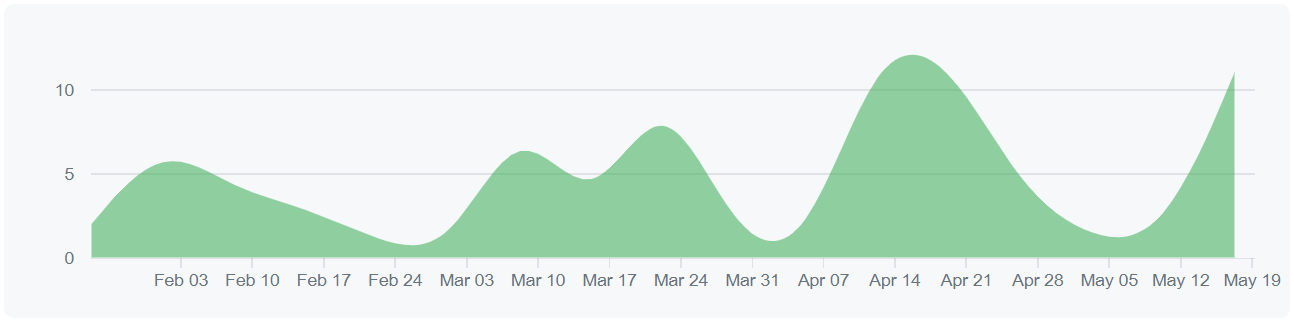
\includegraphics[scale=0.55]{images/contributor_graph_git.PNG}
\caption{Graph des commits}
\label{fig:commits}
\end{figure}

Dans la figure \textcolor{BrickRed}{\ref{fig:commits}}, nous observons, au délà de la préparation et de l'organisation du dépôt, que le nombre de commits était bas pendant la période de fin de février et début de mars. Ceci est dû au fait qu'il s'agit de l'étude préalable consistant surtout en des tâches de lecture.\\
Ensuite, nous constatons la présence d'une autre période de baisse de commits (fin mars et début avril), due aux périodes de rattrapage du premier semestre et de recherche d'une plateforme d'hébergement à \textbf{API} adaptée.\\
Après, les commits augmentent tout au long le mois d'avril où nous entamons la conception et l'implémentation du \textbf{Lister}, et puis la rédaction des rapports et de leurs documents associés.\\
Enfin, les commits baissent encore une fois lors de la période de préparation aux examens finals (fin avril et début mai) pour augmenter vers la fin de mai, avant la date de délai du TER et de ses livrables correspondant.

%graph des commits par jour de la semaine
%
\begin{figure}[!ht]
\hspace*{-4cm}
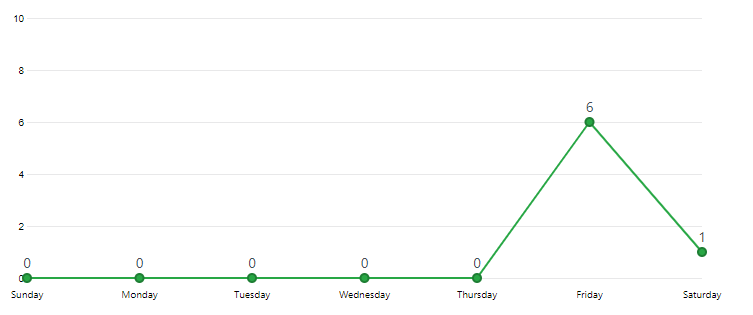
\includegraphics[scale=0.60]{images/contributor_week_feb3.PNG}
\hspace*{1.6cm}
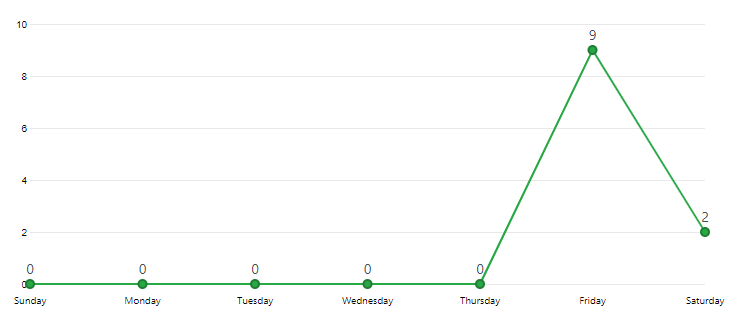
\includegraphics[scale=0.60]{images/contributor_week_march24.PNG}
\caption{Moyenne des commits par jours pour les semaines du 3 février et du 24 mars}
\label{fig:mean_commits}
\end{figure}

Dans la figure \textcolor{BrickRed}{\ref{fig:mean_commits}}, nous observons que les commits étaient souvent effectués les vendredis. En effet, nous avons decidé de se réunir et de travailler ensemble tous les vendredis, le seul jour de la semaine où nous étions tous les trois disponibles simultanément.

\section{Classes et lignes de code}
\begin{table}
  \centering
  \begin{tabular}{|l|c|p{6cm}|}
    \hline
    \textbf{Classe} & \textbf{Lignes de code} & \textbf{Description}\\
    \hline
    \textbf{LaunchpadProxy} & 178 & classe exploitant l'\textbf{API} de \texttt{Launchpad} via un objet proxy désignant une instance du client officiel de \texttt{Launchpad}, afin de récupérer tous les dépôts \textbf{Git} publiquement disponibles.\\
    \hline
    \textbf{LaunchpadGitModel} & 10 & classe définissant le modèle d'un dépôt \textbf{Git} hébergé sur \texttt{Launchpad} au sein de \texttt{Software Heritage}.\\
    \hline
    \textbf{LaunchpadGitLister} & 50 & classe définissant le \textbf{Lister}, implémentant toutes les fonctions requises pour énumérer les dépôts \textbf{Git} hébergés sur \texttt{Launchpad}.\\
    \hline
    \textbf{LaunchpadGitTasks} & 48 & classe définissant les différentes manières dont \textbf{LaunchpadLister} puisse lister les dépôts \textbf{Git} hébergés sur \texttt{Launchpad}, et encapsulant les tâches de \textit{scheduling} et de \textit{loading} responsables de l'ingestion de leur contenu dans l'archive de \texttt{Software Heritage}.\\
    \hline
    \textbf{LaunchpadListerTester} & 21 & classe définissant les tests unitaires à effectuer sur le \textbf{Lister}.\\
    \hline
    \textbf{LaunchpadTaskTester} & 89 & classe définissant les tests unitaires à effectuer sur les tâches du \textbf{Lister}.\\
    \hline
    \textbf{ProxiedLister} & 10 & classe abstraite désignant la \textbf{superclasse} de n'importe quel \textbf{Lister} à intégrer à \texttt{Software Heritage}, possédant les mêmes exigences que celui de \texttt{Launchpad}, (\textit{i.e. intégrant un proxy qui agira comme intermédiaire entre l'\textbf{API} et le \textbf{Lister}}).\\
    \hline
    \textbf{WebApiProxy} & 49 & Une interface contenant les \textbf{signatures des méthodes} requises par la classe d'un \textbf{proxy} utilisé par un \textbf{ProxiedLister}.\\
    \hline
  \end{tabular}
\end{table}

\newpage

\section{Temps de Travail}
Concernant le temps de travail, nous estimons (approximativement) :
\begin{itemize}
\item 110 heures sur l'étude préalable du projet ;
\item 60 heures pour la recherche de plateformes d'hébergement de code et pour tester leurs \textbf{API}s ;
\item 110 heures pour le developpement du code ;
\item 20 heures pour la documentation et les rapports ;
\end{itemize}

\noindent Nous estimons encore environ 30 heures de travail, portant sur l'écriture du rapport du TER et de la présentation.

\chapter{Conclusion}
Dans ce projet, nous avons essayé d'appliquer les techniques proposées par le module de conduite de projets, afin de baliser et maîtriser le projet le plus possible. En particulier, nous avons créé un planning prévisionnel en utilisant un diagramme de Gantt, nous avons évalué le profile de risque de notre projet et nous avons concrétisé une stratégie de développement complète.

En outre, le fait que nous n'avions été introduit à la méthodologie de développement agile qu'après avoir commencé le module TER, nous a empêché de l'adopter dès le début. Par ailleurs, notre émulation d'un tableau de bord via les \textit{meeting minutes} était assez utile, certes, mais nous aurons dû la remplacer par un tableau de bord digital tel que celui offert par l'application \texttt{Trello}.

En définitive, le projet nous a rapporté une expérience conséquente en terme de gestion de projets par application directe des notions apprises en cours, mais également en terme de nouvelles technologies assimilées.
\end{document}
